\documentclass[12pt]{article}
\usepackage{fullpage,amsmath,amssymb,graphicx}

\usepackage{setspace}
\spacing{1}

\usepackage{textpos}
\usepackage{tikz}
\usepackage{pgf}
\usepackage{amssymb}
\usepackage{enumerate}
\usepackage{xcolor}
\usepackage{graphicx}
\usepackage{subcaption}
\usepackage{tabularx}
\usepackage{colortbl}
\usepackage{multicol}
\usepackage{longtable}
\usepackage{hyperref}


\definecolor{encabezado}{rgb}{0.74, 0.83, 0.9}

\begin{document}

\hfill\\
\rule{\textwidth}{1.5pt}

\begin{minipage}[t]{85mm}
  \begin{tabular}{l}
    \textbf{\large Instituto Tecnológico de Costa Rica} \\  
    \textbf{Escuela de Ingeniería Electrónica} \\
    \textbf{Trabajo Final de Graduación} \\
    \textbf{Proyecto:} Método basado en aprendizaje reforzado \\para el control automático de una planta no lineal. \\
    \textbf{Estudiante:} Oscar Andrés Rojas Fonseca \hspace{3cm}\rule{4.5cm}{1.5pt}\\
    I Semestre 2024 \hspace{8.5cm}\textbf{Firma del asesor}
  \end{tabular}
\end{minipage}
\hfill\\
\rule{\textwidth}{1.5pt}


\section*{Bitácora de trabajo}

%\begin{table}[h]
\begin{minipage}[h]{\textwidth}
	\centering
	\begin{tabularx}{\textwidth}{|p{2cm}|X|X|p{2cm}|} 
		\hline
		\rowcolor{encabezado}
		\textbf{Fecha} & 
		\textbf{Actividad} & 
		\textbf{Anotaciones} & 
		\textbf{Horas dedicadas} \\ \hline
		% ***************************************************************
		05/02/2024 & 
		$\mathbf{1}.$ Estudio de a teoría de control para el péndulo amortiguado a hélice (PAMH). & 
		$a)$ Consulta a bibliografía de control automático: Nise (2020) y Ogata (2003). \newline $b)$ Revisión de material multimedia de Anibal Ruiz-Barquero referente al PAMH vía Youtube. \newline & 
		3 horas \\
	 	% ***************************************************************
	 	06/02/2024 & 
	 	$\mathbf{2}.$ Estudio de la teoría de aprendizaje reforzado (RL). &
	 	$a)$ Consulta a libros de texto como \textit{Data-Driven Science and Engineering} (Brunton y Kutz, 2021). \newline $b)$ Revisión de material multimedia de Steven Brunton vía Youtube. \newline & 
	 	3 horas \\
	 	% ***************************************************************
	 	06/02/2024 & 
	 	$\mathbf{3}.$ Revisión bibliográfica de algoritmos de aplicación de aprendizaje automático. & 
	 	$a)$ Consulta al libro \textit{Reinforcement Learning: An introduction} (Sutton y Barto, 2020) para mayor detalle. \newline $b)$ Revisión de otros métodos de aprendizaje automático. \newline $c)$ Ejemplos de implementación de las redes neuronales recurrentes (RNN) por Patrick Loeber vía Youtube y la tésis de graduación de Jorge Brenes. & 
	 	3 horas \\
	 	
	 	\hline
	\end{tabularx}
\end{minipage}	 	
	 	
	 	% ***************************************************************
\hfill\\
\begin{minipage}[h]{\textwidth}
	\centering
	\begin{tabularx}{\textwidth}{|p{2cm}|X|X|p{2cm}|} 
		\hline		
		
	 	07/02/2024 & 
	 	$\mathbf{4}.$ Revisión de repositorios en línea de métodos de aplicación de aprendizaje automático. & 
	 	$a)$ Búsqueda preliminar de repositorios generales de RL mediante Github. \newline $b)$ Selección de códigos con enfoques similares al control del PAMH. \newline & 
	 	5 horas \\
	 	% ***************************************************************
	 	09/02/2024 & 
	 	$\mathbf{5}.$ Creación del ambiente de trabajo anaconda para montaje de la red neuronal mimetizadora (RNAM). & 
	 	$a)$ Revisión de bibliotecas utilizadas por el código base de la RNAM.\newline $b)$ Instalación/revisión de versiones adecuadas de \textit{Python}, \textit{ArgumentParser}, \textit{Numpy}, \textit{Matplotlib}, \textit{TensorFlow} y \textit{Weights\&Biasis}.\newline & 
	 	2 horas \\
	 	% ***************************************************************
	 	09/02/2024 & 
	 	$\mathbf{6}.$ Pruebas de funcionamiento de la red neuronal mimetizadora (Synthetic-PAHM.py). & 
	 	$a)$ Estudio del código de la RNAM. \newline $b)$ Error en el proceso por falta de cuenta y permisos del autor en W\&B. \newline $c)$ Creación de cuenta y proyecto en W\&B. \newline & 
	 	3 horas \\
	 	% ***************************************************************
	 	09/02/2024 & 
	 	$\mathbf{7}.$ Estudio del funcionamiento de la herramienta Weights \& Biases (W\&B). & 
	 	$a)$ Revisión de material en línea sobre el uso de W\&B. \newline $b)$ Ejemplos de implementación de W\&B. & 
	 	2 horas \\
	 	% ***************************************************************
	 	\hline
		\multicolumn{3}{|r|}{Total de horas de trabajo:} & 21 horas \\ 
	 	\hline                 
	\end{tabularx}
\end{minipage}
%\end{table}

% *****************************************************************************
% *****************************************************************************
% *****************************************************************************

\section*{Contenidos de actividades}

\subsection*{Resumen de teoría PAMH}

El péndulo amortiguado a hélice corresponde a una planta de laboratorio compuesta de un motor con hélice controlado por torque, una masa pequeña, péndulo y soportes de aluminio de baja fricción. Un modelo simplificado del sistema se muestra en la Figura \ref{fig:modpen} \cite{PAMH1}.

\begin{figure}[h]
	\centering
	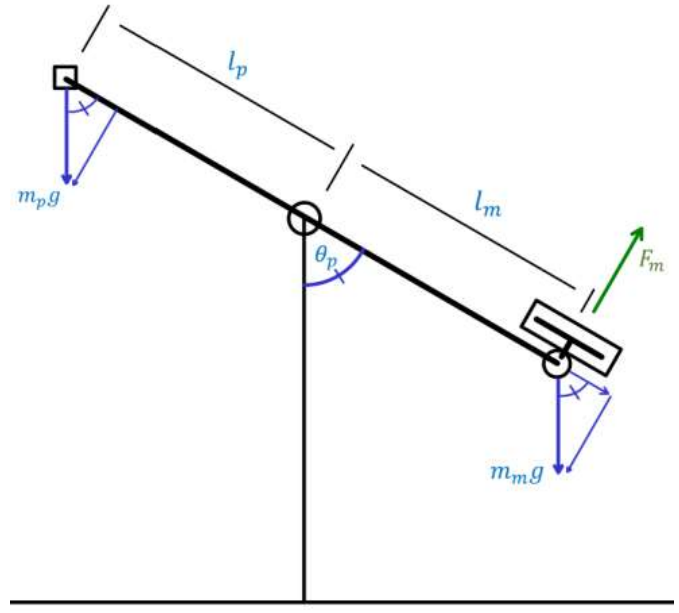
\includegraphics[scale=0.3]{Fig/ModeloPendulo.png}
	\caption{Modelo simplificado del PAMH.}
	\label{fig:modpen}
\end{figure}

El objetivo de dicho sistema es controlar la magnitud del ángulo $\theta_p$, únicamente ejerciendo torque al accionar a una distancia $l_m$ el motor con una fuerza $F_m$ y movimiento de su masa $m_m$, mientras a una distancia de $l_p$ del centro se encuentra una masa $m_p$ que contrarresta el movimiento.

De manera que al analizar el sistema con sumatoria de torques se obtiene la constante de rosamiento central $B$ (en caso de existir) junto con la inercia ejercida $J_p$. Por lo tanto, se definen las variables de estado siguientes y sus ecuaciones de estado mostradas en \ref{ecu:ecuestados} \cite{ControlModerno}.

\[x_1 = \theta_p \qquad x_2 = \dot{\theta}_p \qquad y = x_1 = \theta_p\]
\begin{equation}
	\left \{ \begin{array}{lcc} \dot{x}_1 = x_2 \\ \\ \dot{x}_2 = -\dfrac{B}{J_p} x_2 + (m_p l_p -m_m l_m)\dfrac{g}{J_p}sen(x_1) +\dfrac{l_m}{J_p}F_m \end{array} \right.
	\label{ecu:ecuestados}
\end{equation}



\subsection*{Resumen de teoría RL}

Al estudiar el concepto de aprendizaje reforzado y los diferentes métodos y algoritmos que corresponden a este tipo de aprendizaje automático, se obtiene el resumen de la Figura \ref{fig:teoriaRL}, en donde se muestra que las principales secciones son el RL basado en modelo y el libre de modelo. De igual forma se cuenta con el aprendizaje reforzado profundo (DRL), una combinación y reestructuración de métodos de cada subdivisión \cite{DataScience}.

\begin{figure}[hh]
	\centering
	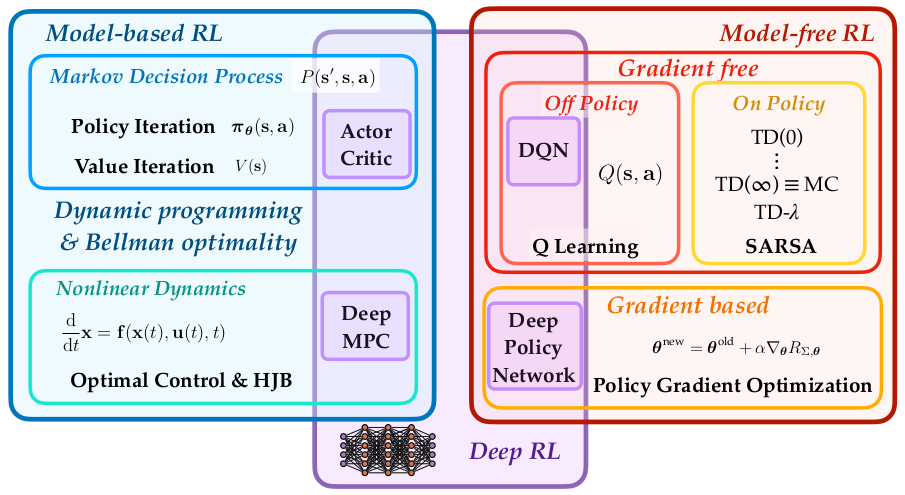
\includegraphics[scale=0.35]{Fig/CatRL.png}
	\caption{Resumen de categorización del RL \cite{DataScience}.}
	\label{fig:teoriaRL}
\end{figure}


De igual manera, los avances en la investigación de diferentes métodos como las redes neuronales recurrentes (RNN), ejemplificado por Mamba \cite{Mamba}, ha mostrado la capacidad de optimización del desempeño de estas para llegar a competir con los modelos basados en \textit{Transformer}.


\subsection*{Ambiente de trabajo anaconda para la RNAM}

Luego de una revisión rápida del código perteneciente al repositorio del trabajo de Jorge Brenes, se instalaron versiones de bibliotecas necesarias para el funcionamiento de los registros, resultando en una lista simplificada como la mostrada en la Figura \ref{fig:capturaenv}.

\begin{figure}[h]
	\centering
	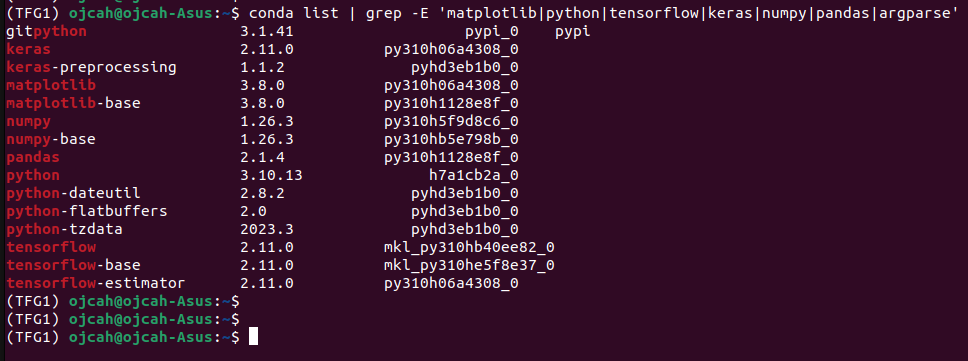
\includegraphics[scale=0.43]{Fig/CapturaEnv.png}
	\caption{Lista simplificada de bibliotecas del \textit{environment} TFG1.}
	\label{fig:capturaenv}
\end{figure}



\newpage

\section*{Referencias}
\renewcommand\refname{}
\bibliographystyle{IEEEtran}
\bibliography{references}





\end{document}